\item In the arrangement shown in Fig. 1.24 the masses \( m \) of the bar and \( M \) of the wedge, as well as the wedge angle \(\alpha\), are known.
    \begin{center}
        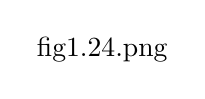
\begin{tikzpicture}
            \node at (0, 0) {{fig1.24.png}};
        \end{tikzpicture}
    \end{center}
The masses of the pulley and the thread are negligible. The friction is absent. Find the acceleration of the wedge \( M \).\begin{solution}
    \begin{center}
        \begin{tikzpicture}
            \pic at (0, 0) {frame=3cm};
        \end{tikzpicture}
    \end{center}
    
    \begin{align*}
        \intertext{On the basis of force diagram, it is obvious that the wedge \(M\) will move towards right and the block will move down along the wedge. As the length of the thread is constant, the distance travelled by the block on the wedge must be equal to the distance travelled by the wedge on the floor. Hence \(ds_{mM} = ds_M\). As \(\vec{v}_{mM}\) and \(\vec{v}_M\) do not change their directions and acceleration, that’s why \(\vec{w}_{mM}\uparrow\uparrow\vec{v}_{mM}\) and \(\vec{w}_M\uparrow\uparrow\vec{v}_M\) and \(\vec{w}_{mM} = w\) (say) and accordingly the diagram of kinematical dependence is shown in figure.}
        \intertext{As \(\vec{w} = \vec{w}_M + \vec{w}_{mM}\) so from triangle law of vector addition}
        w_m &= \sqrt{w^2_M + w^2_mM - 2w_Mw_{mM}\cos\alpha}=w\sqrt{2(1-\cos\alpha)}\tag{1}\\
        \intertext{From \(F_x=mw_{x_0}\) (for the wedge),}
        T-T\cos\alpha+N\sin\alpha &= Mw\tag{2}\\
        \intertext{For the bar m let us fix x-y coordinate system in the frame of ground. Newton's law in projection form along x- and y-axes (see figure) gives}
        mg\sin\alpha-T &= mw_{m(x)} = m[w_{mM(x)}+w_{M(x)}]\\
        &= m[w_{mM}+w_M\cos(\pi-\alpha)] = mw(1-\cos\alpha)\tag{3}\\
        mg\cos\alpha-N &= mw_{m(y)} = m[w_{mM(y)}+w_M(y)] = m[0+w\sin\alpha]\tag{4}
        \intertext{Solving the above equations simultaneously, we get}
        w &= \dfrac{mg\sin\alpha}{M+2m(1-\cos\alpha)}
        \intertext{Note: We can study the motion of the block m in the frame of wedge also, alternately we may solve this problem using conservation of mechanical energy.}
    \end{align*}
\end{solution}